\documentclass[11pt, a4paper]{article}
\usepackage{graphicx}
\usepackage{amsmath}
\usepackage{listings}

\title{Assignment 7: Laplace transform}
\author{G Ch V Sairam , EE19B081}
\date{16-04-2021}

\begin{document}		
		
\maketitle
\section*{Introduction}
In this assignment , we learn to use the scipy.signal module in python to analyze Linear Time-Invariant systems. We use 3 systems: A osciallator undergoing forced damping , A coupled differential equation system and an RLC filter. All these systems only have rational transfer functions.

\section*{Question 1}
We are given a forced oscillatory system with 0 initial conditions.
\begin{equation}
    \ddot x + 2.25x = f(t)
\end{equation}
Converting into the laplace domain , we get
\begin{equation}
    s^2 X(s) + 2.25X(s) = F(s)
\end{equation}
Then , X(s) can be written as,
\begin{equation}
    X(s) = \frac{F(s)}{s^2+2.25}
\end{equation}
We then find out the impulse response of $X(s)$ and plot it.

\lstinputlisting[language=Python,firstline=13,lastline=21]{EE19B081_assign7.py}

\begin{figure}[!tbh]
\centering
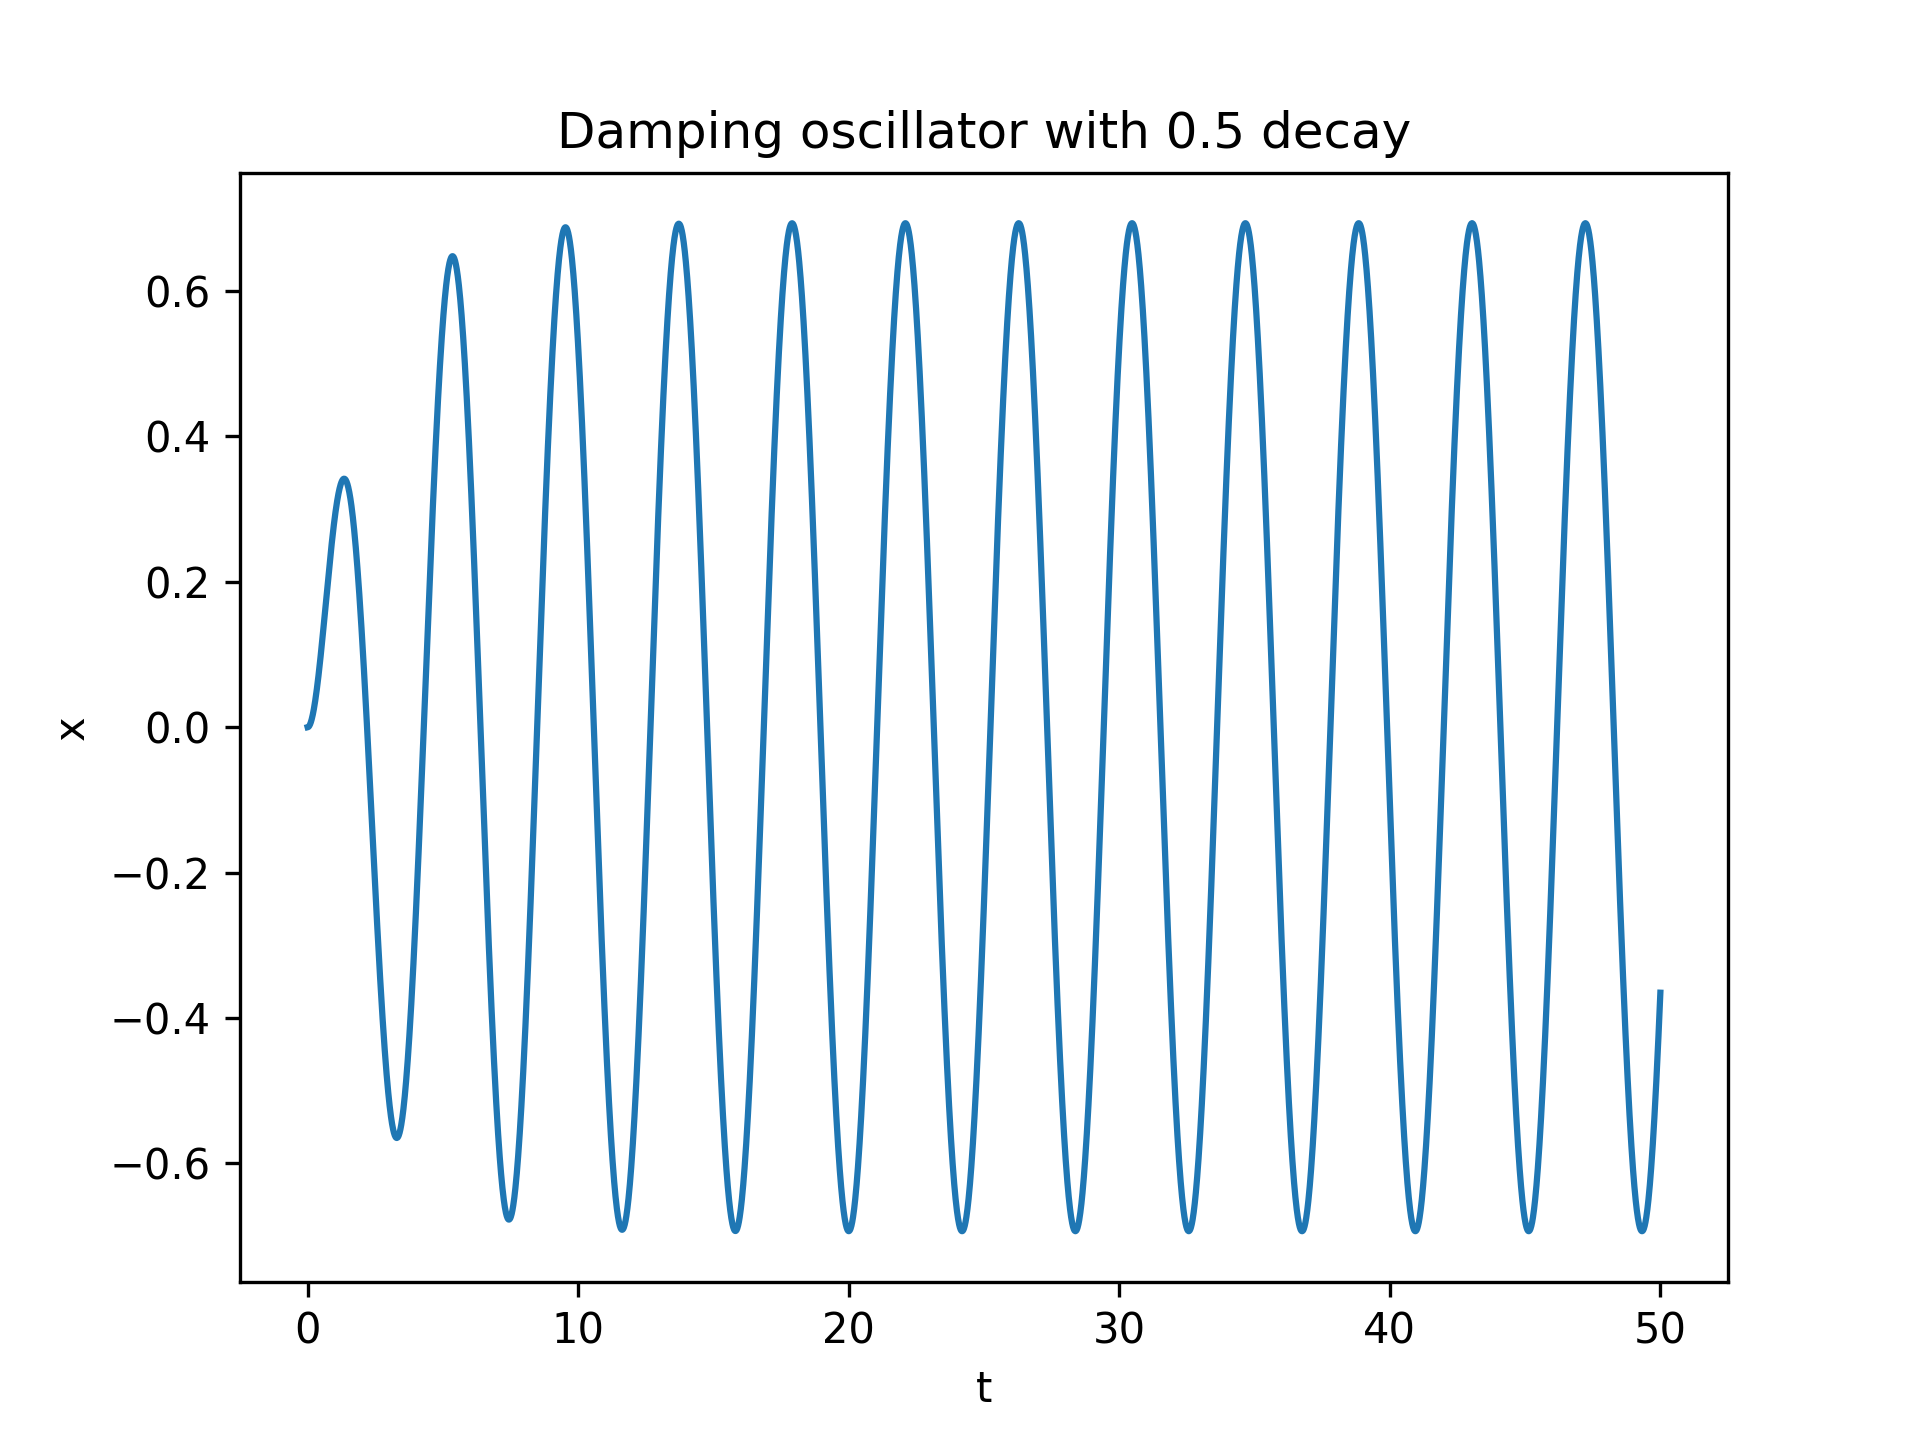
\includegraphics[scale=0.55]{assgn7_plot1.png} 
\caption{Damping oscillator with decay=0.5}
\label{fig1}
\end{figure}

\section*{Question 2}
We do repeat the above block with a different amount of delay , 0.05.

\lstinputlisting[language=Python,firstline=24,lastline=27]{EE19B081_assign7.py}

\begin{figure}[!tbh]
\centering
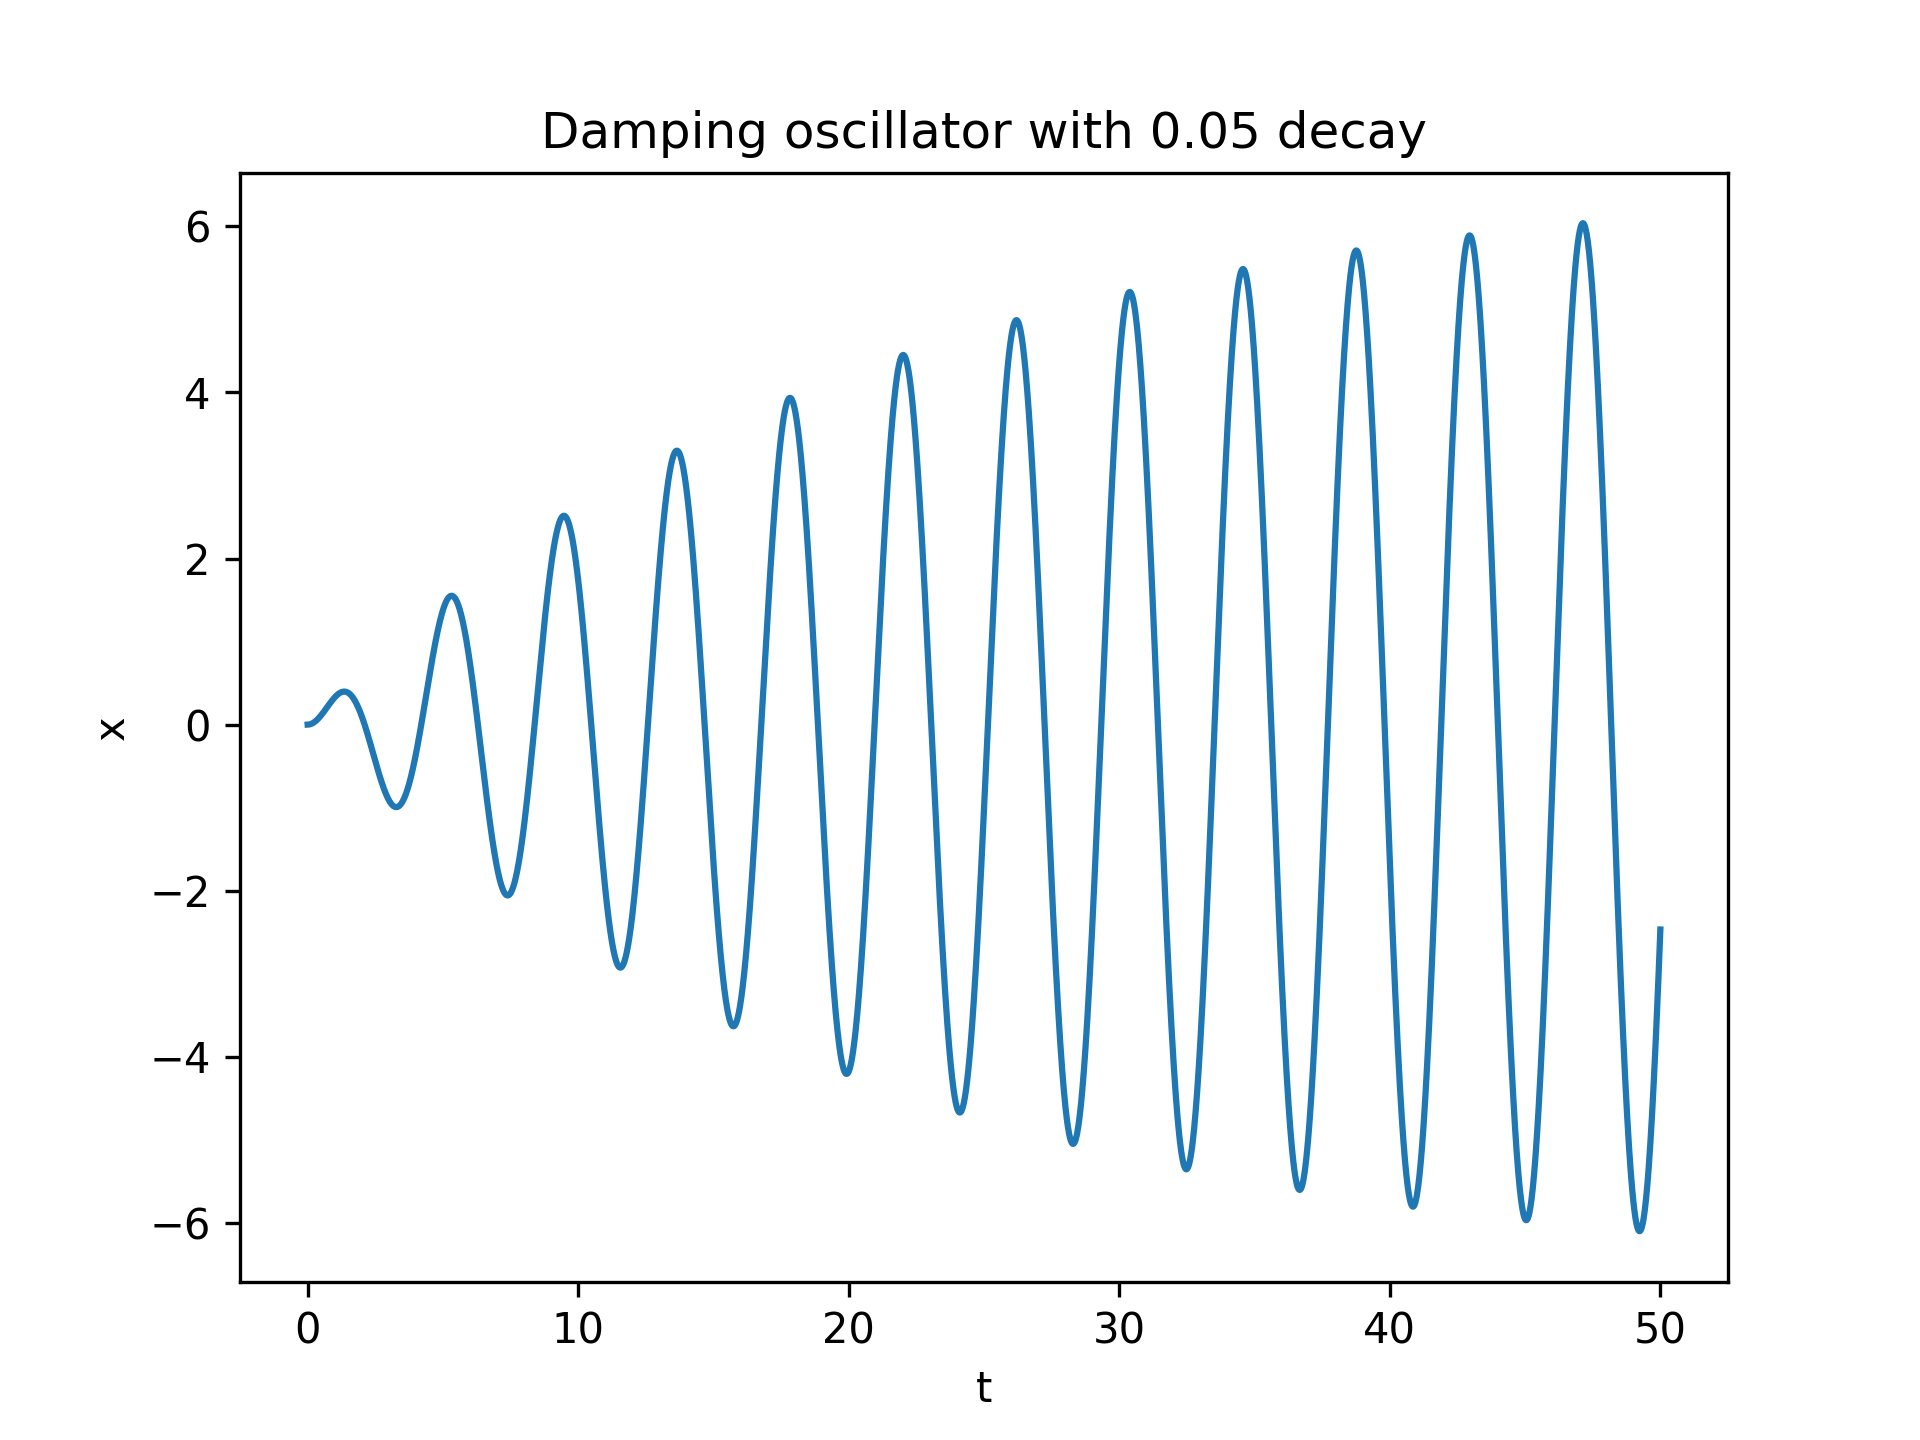
\includegraphics[scale=0.5]{assgn7_plot2.png} 
\caption{Damping oscillator with decay=0.05}
\label{fig2}
\end{figure}

We notice that the result is very similar to that of question 1, except with a
different amplitude. This is because the system takes longer to reach a steady
state.

\section*{Question3}
We now vary the frequency keeping the delay the same(i.e;-0.05). We plot the graphs with the frequencies 1.4,1.45,1.5,1.55 and 1.6 Hz.

\begin{figure}[!tbh]
\centering
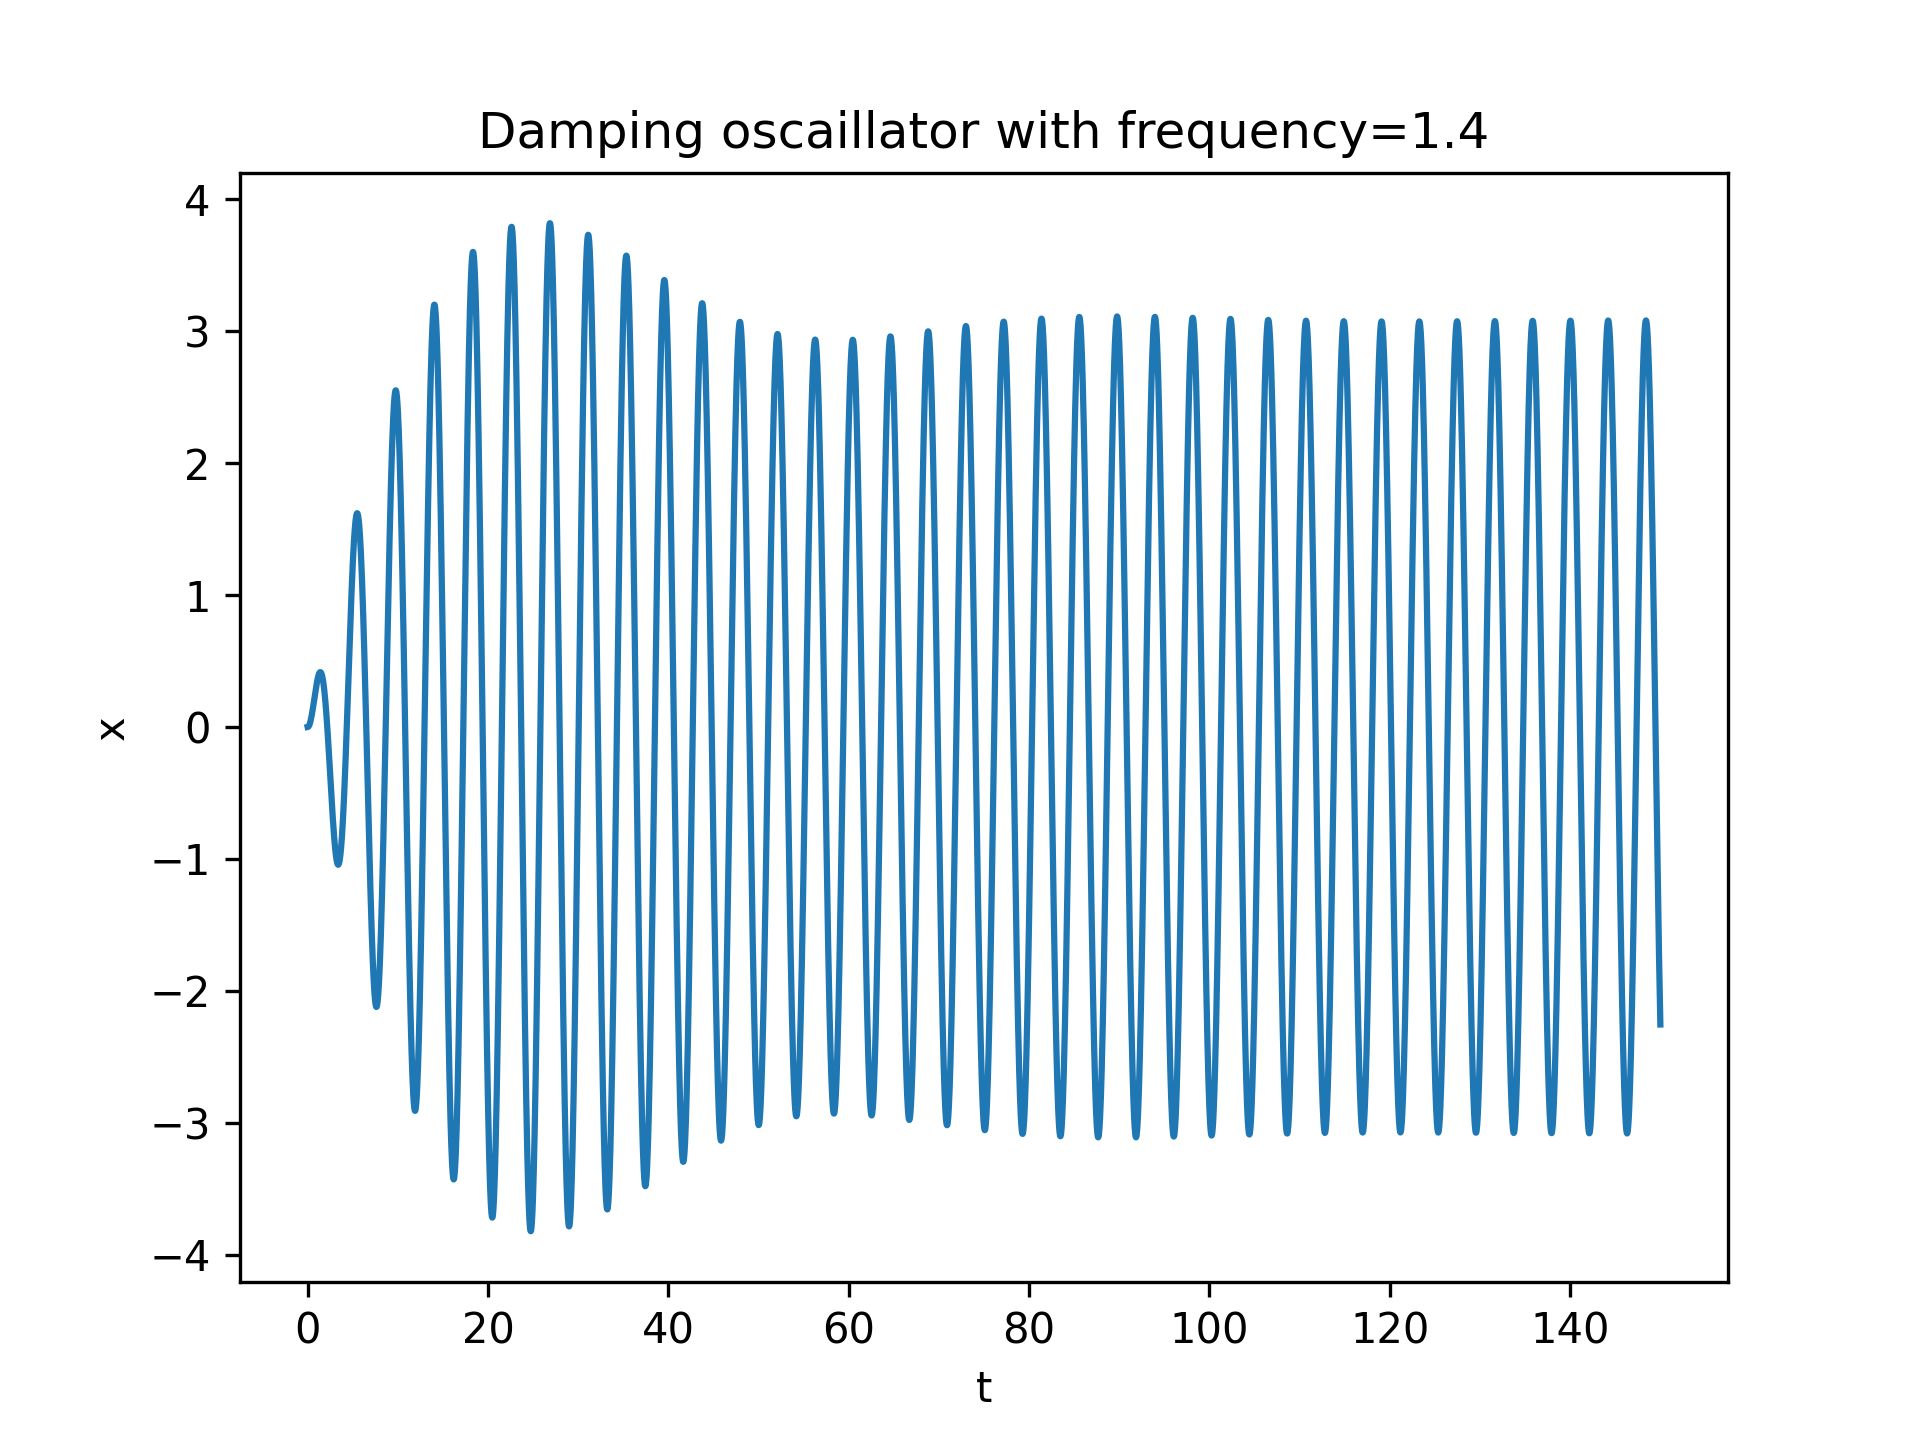
\includegraphics[scale=0.65]{assgn7_plot3.png} 
\caption{Damping oscillator with decay=1.4}
\label{fig3}
\end{figure}

\begin{figure}[!tbh]
\centering
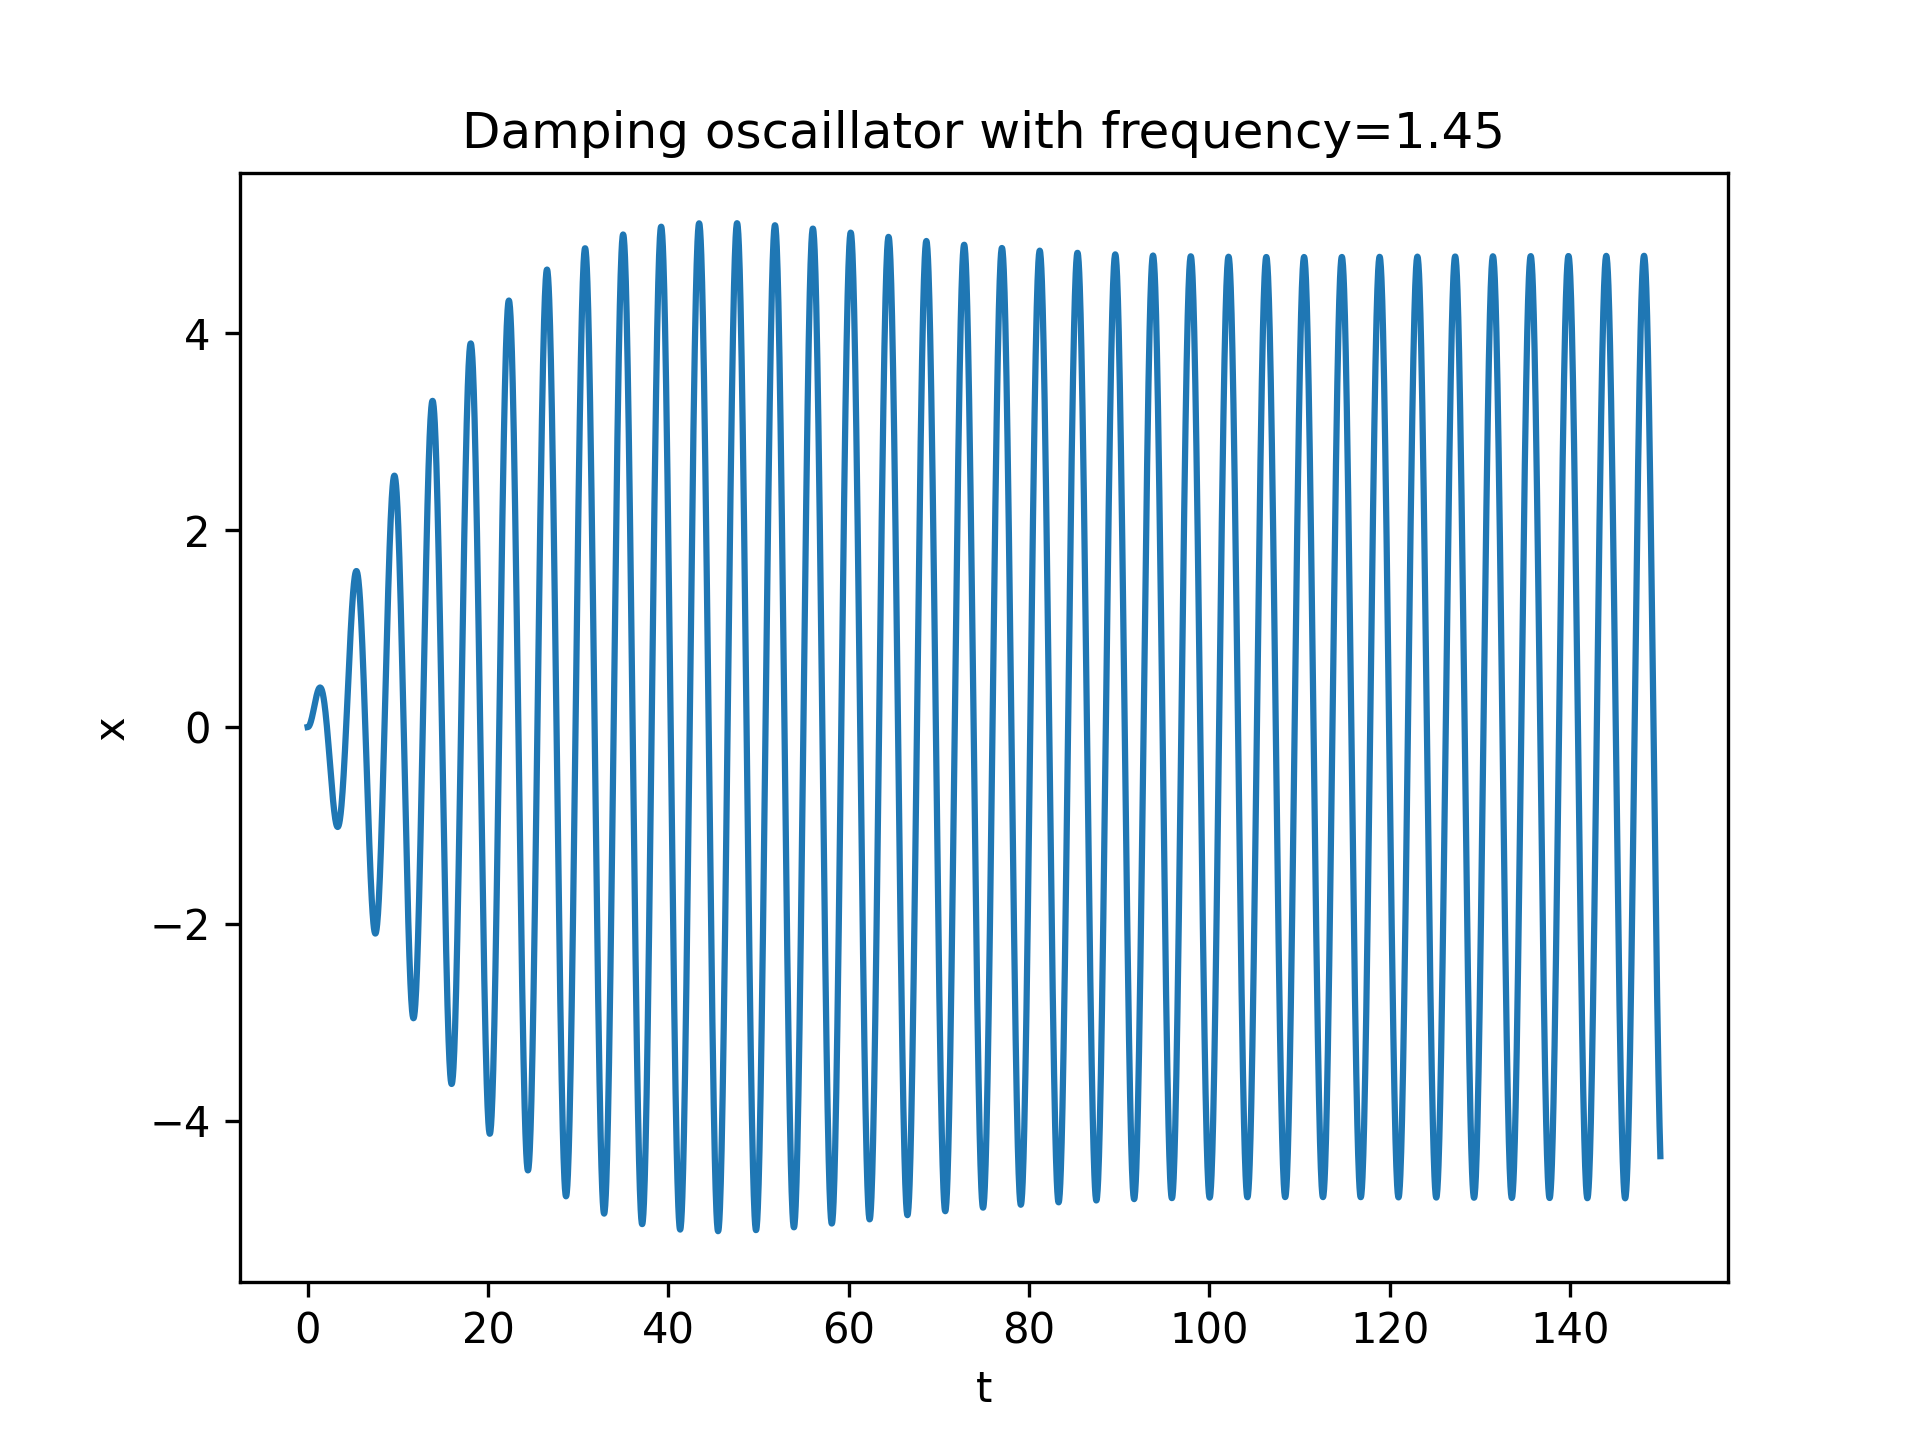
\includegraphics[scale=0.65]{assgn7_plot4.png} 
\caption{Damping oscillator with decay=1.45}
\label{fig4}
\end{figure}

\begin{figure}[!tbh]
\centering
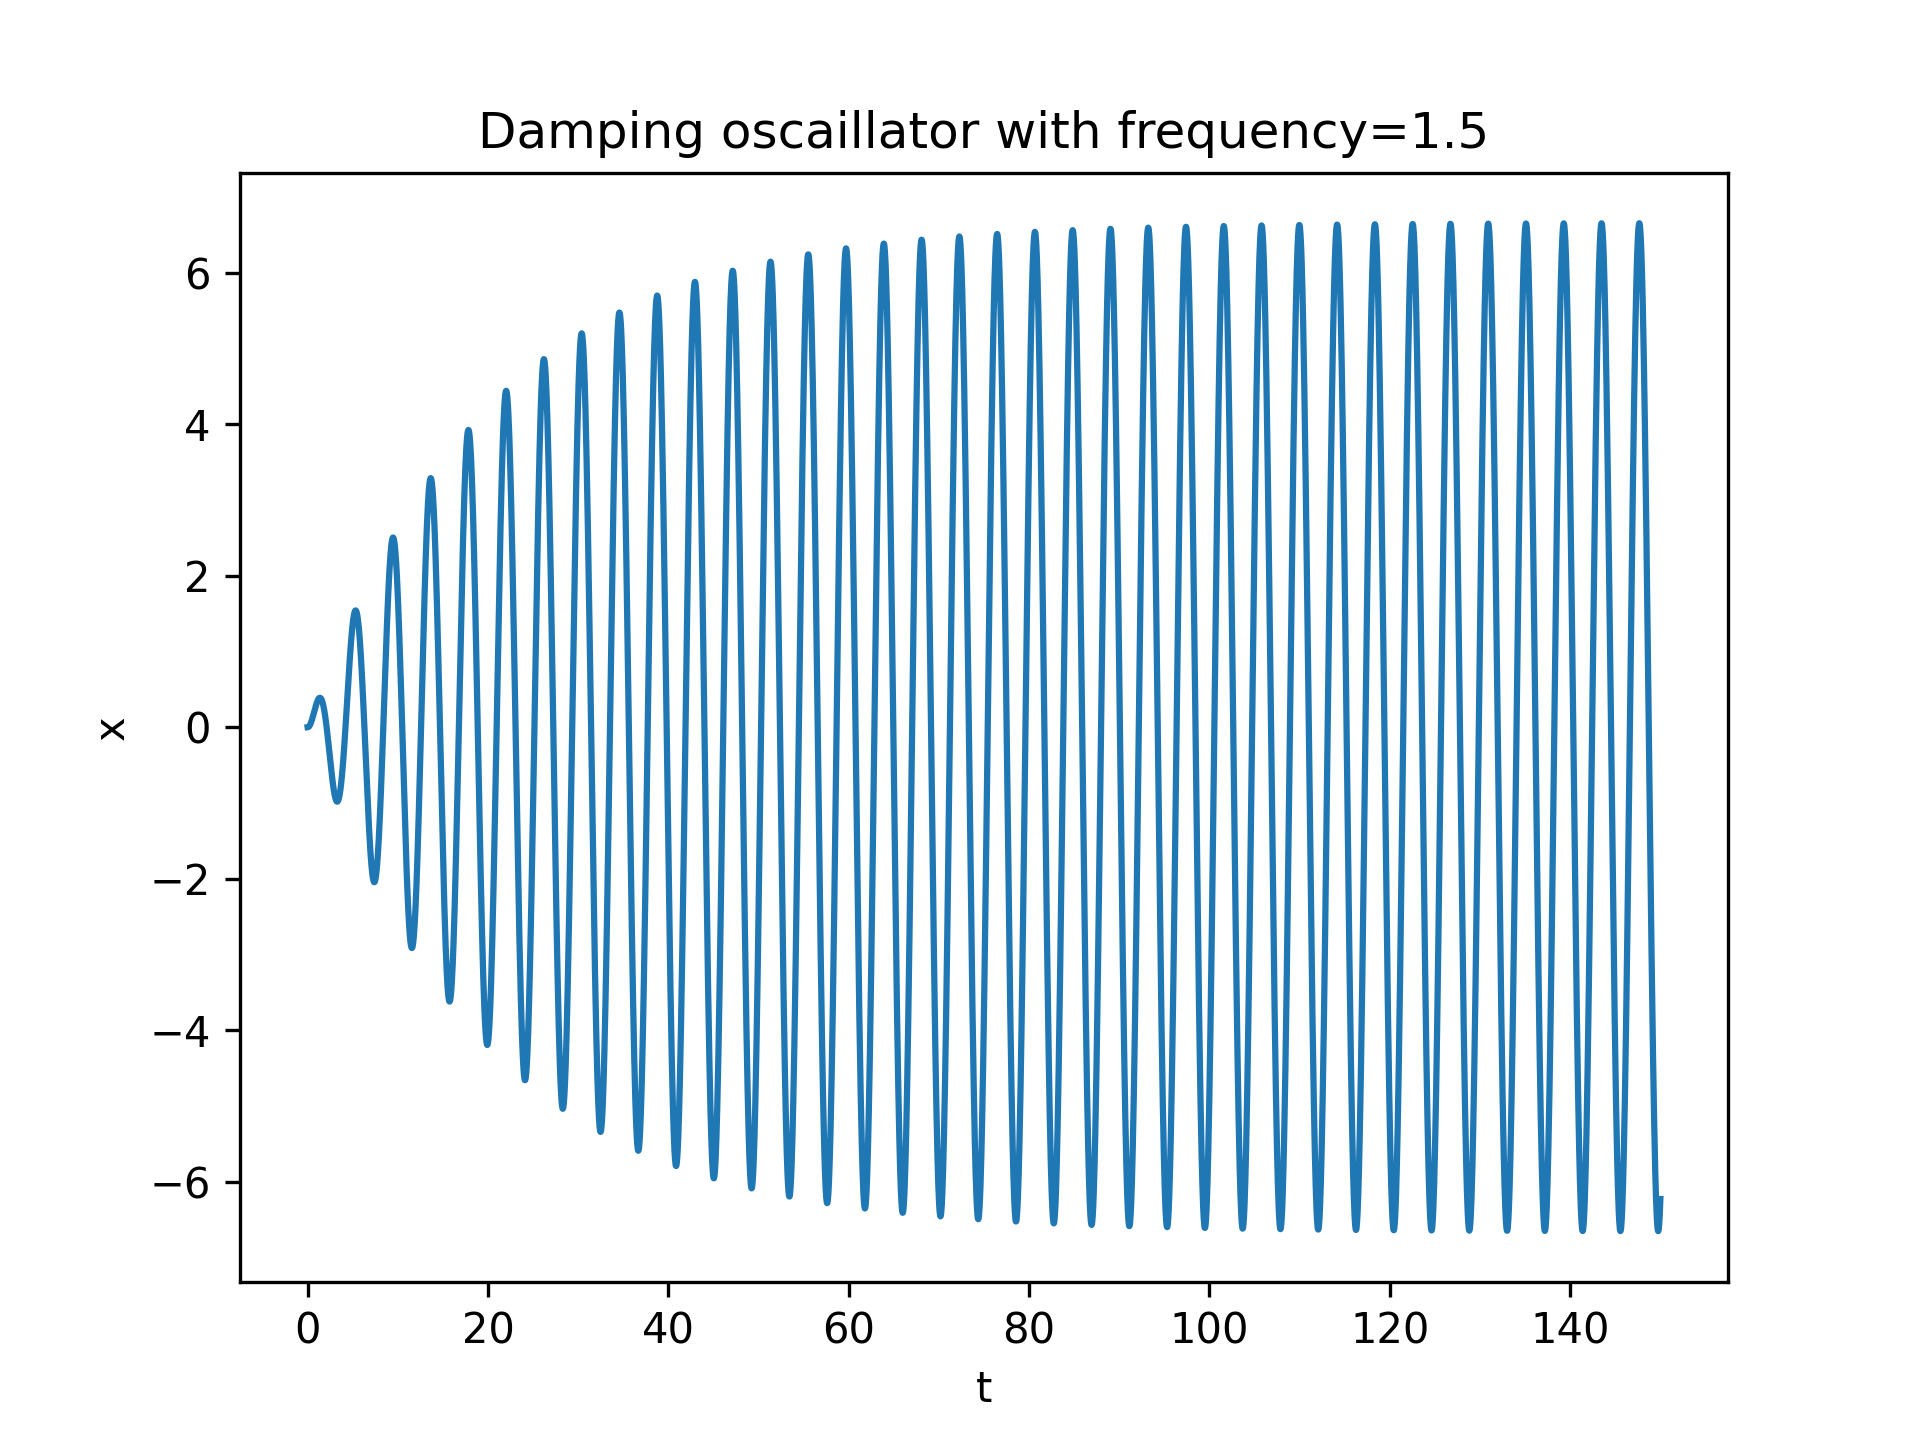
\includegraphics[scale=0.75]{assgn7_plot5.png} 
\caption{Damping oscillator with decay=1.5}
\label{fig5}
\end{figure}

\begin{figure}[!tbh]
\centering
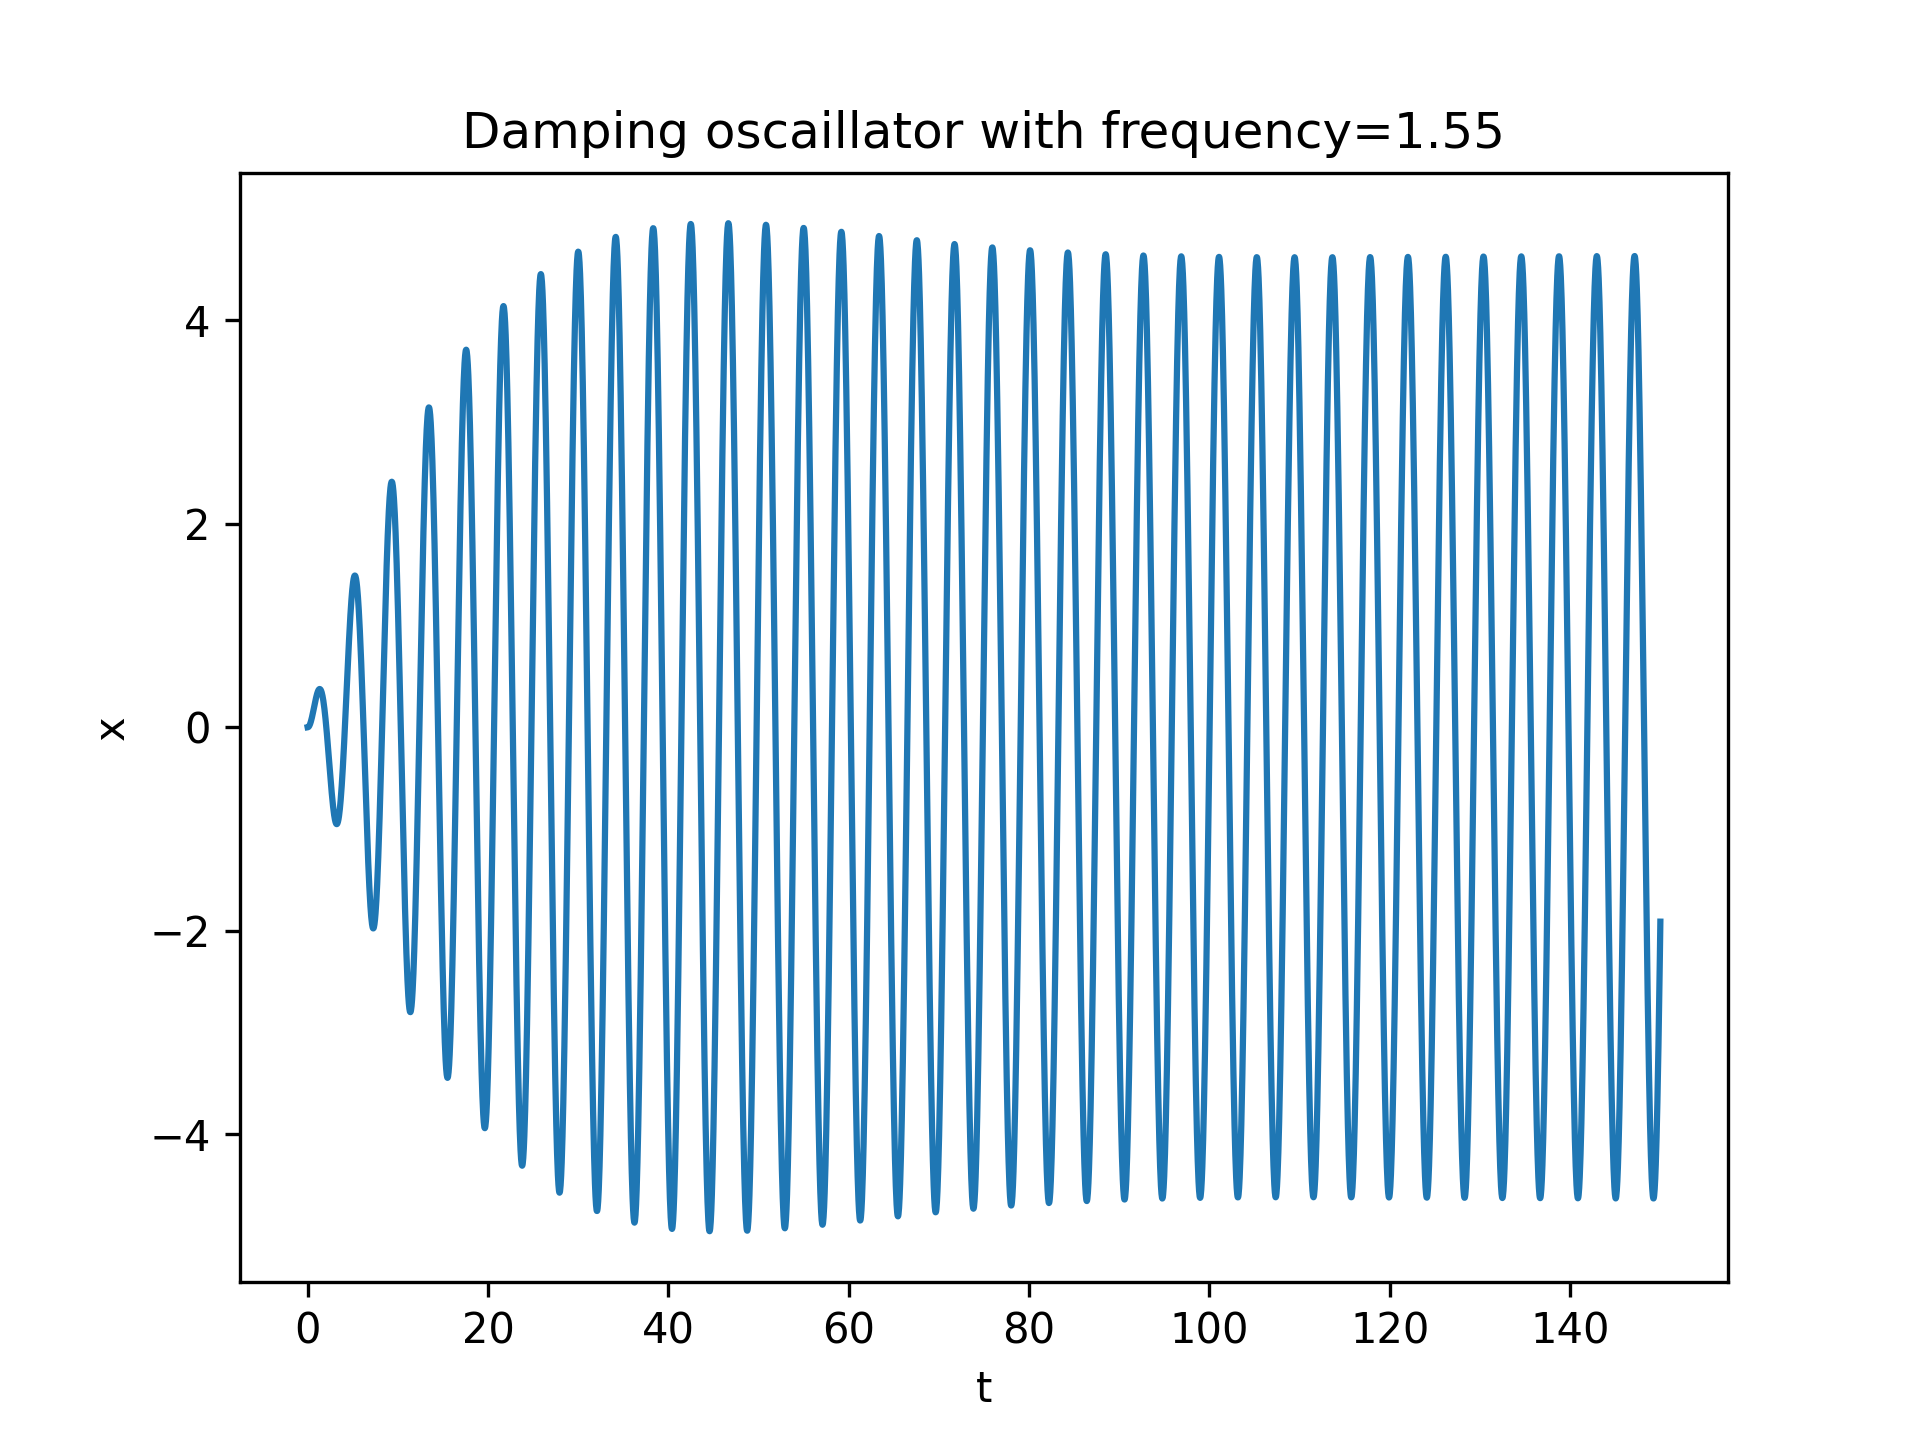
\includegraphics[scale=0.7]{assgn7_plot6.png} 
\caption{Damping oscillator with decay=1.55}
\label{fig6}
\end{figure}

\begin{figure}[!tbh]
\centering
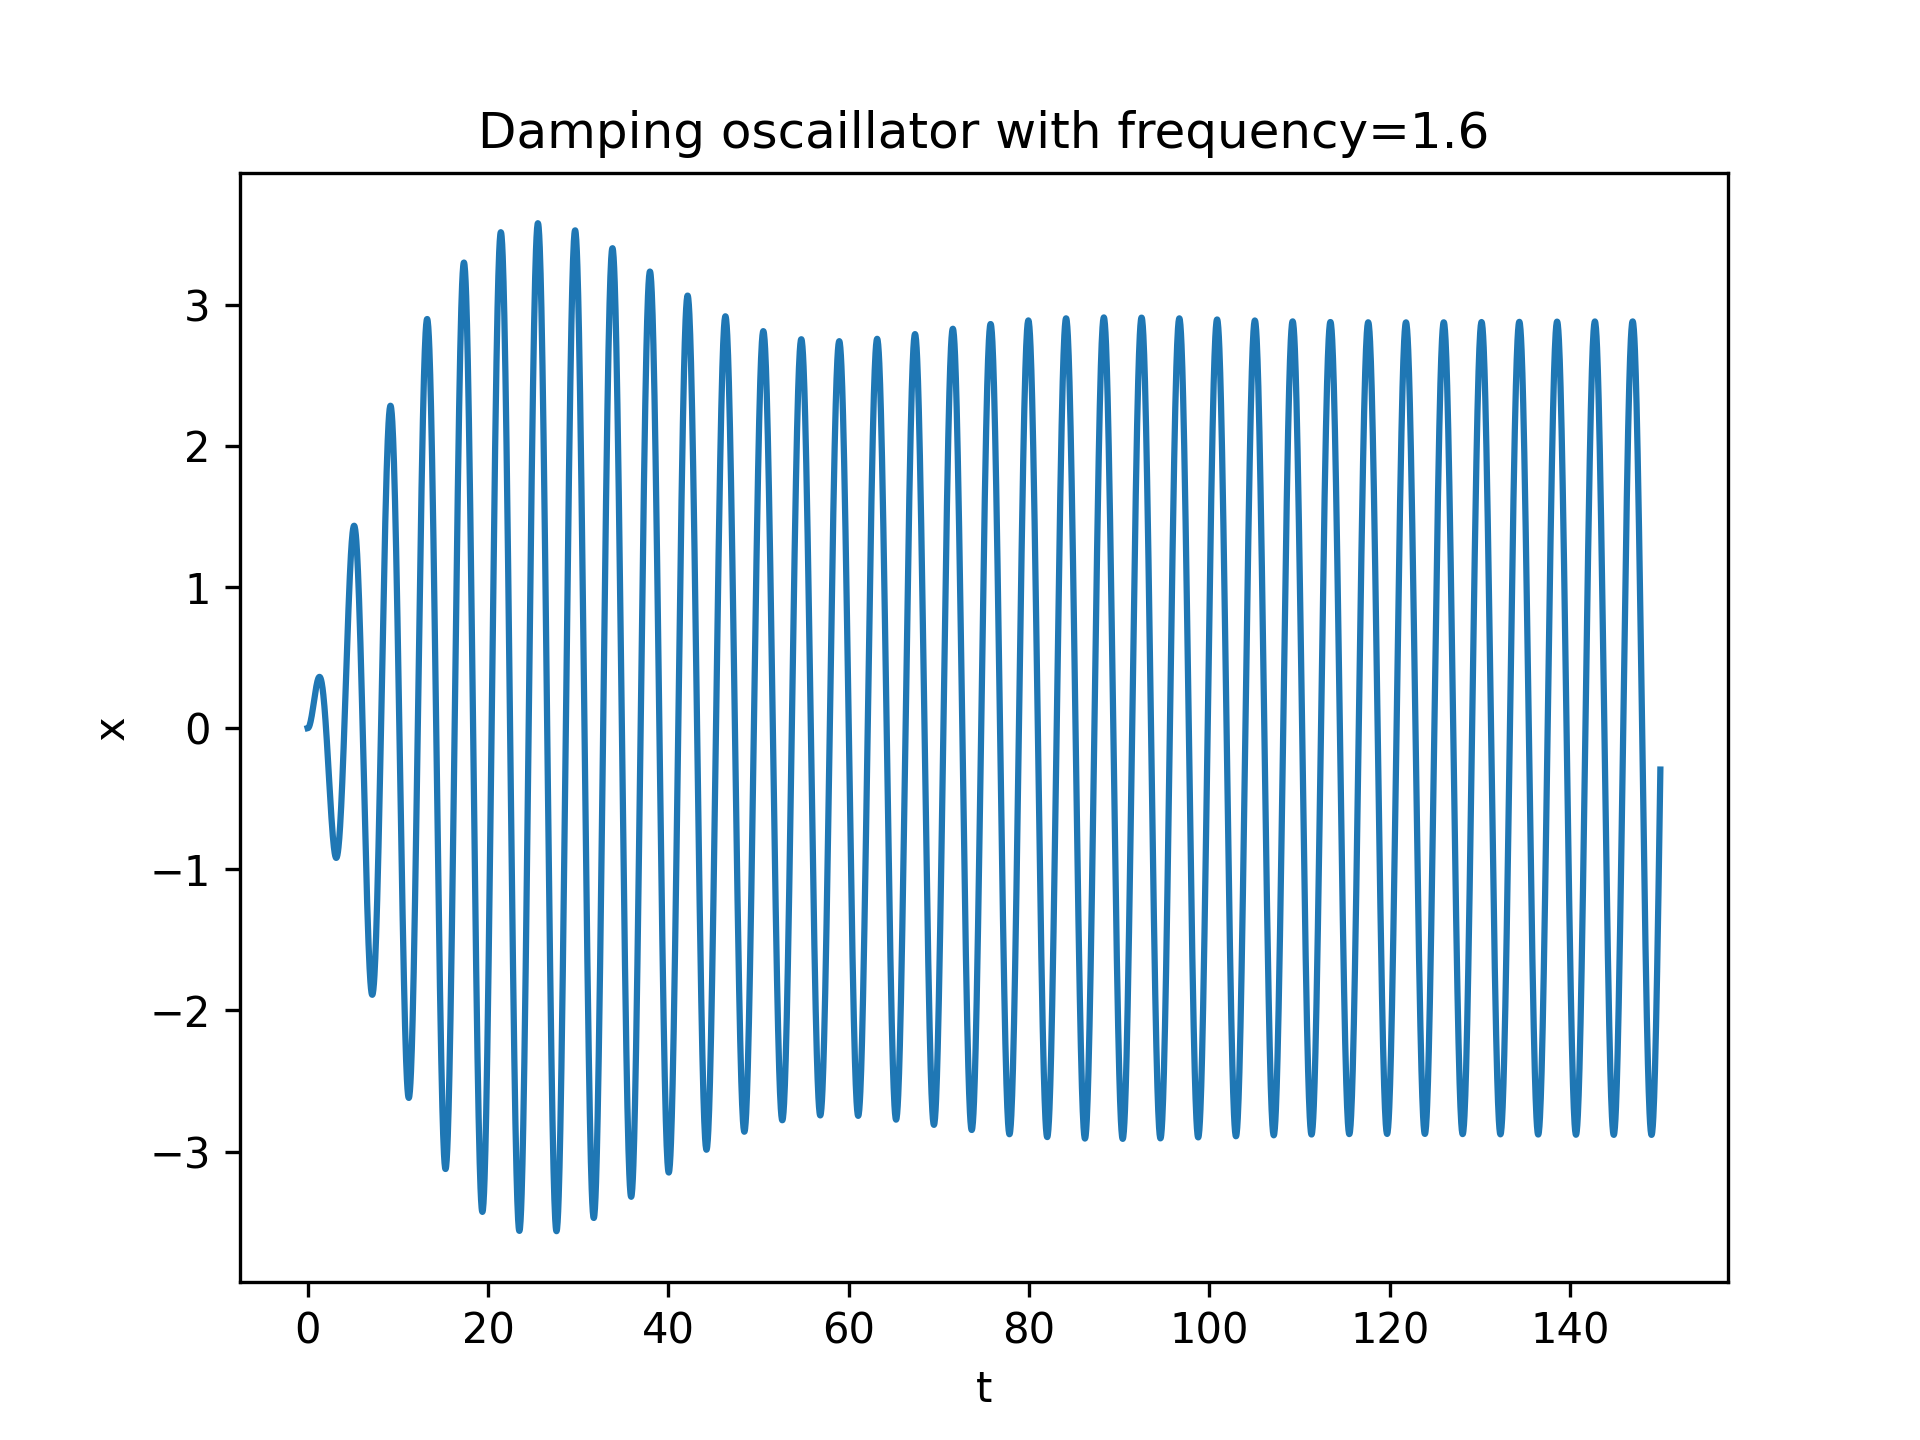
\includegraphics[scale=0.65]{assgn7_plot7.png} 
\caption{Damping oscillator with decay=1.6}
\label{fig7}
\end{figure}

We notice that the amplitude is maximum at frequency=1.5 Hz

\section*{Question 4}
Here , we are given a coupled system of differential equations.
The given equations are:
\begin{equation}
    \ddot x + (x-y) = 0
\end{equation} 
\begin{equation}
    \ddot y + 2(y-x) = 0
\end{equation}
Transforming these equations into laplace domain , we get:

$s^2$X(s)+X(s)-Y(s)=0

$s^2$Y(s)+2(Y(s)-X(s))=0

Solving these equations , we get the solution:
\begin{equation}
    X(s) = \frac{s^2+2}{s^3 + 3s}
\end{equation}
\begin{equation}
    Y(s) = \frac{2}{s^3 + 3s}
\end{equation}
We plot their impulse responses.
\lstinputlisting[language=Python,firstline=47,lastline=52]{EE19B081_assign7.py}

\begin{figure}[!tbh]
\centering
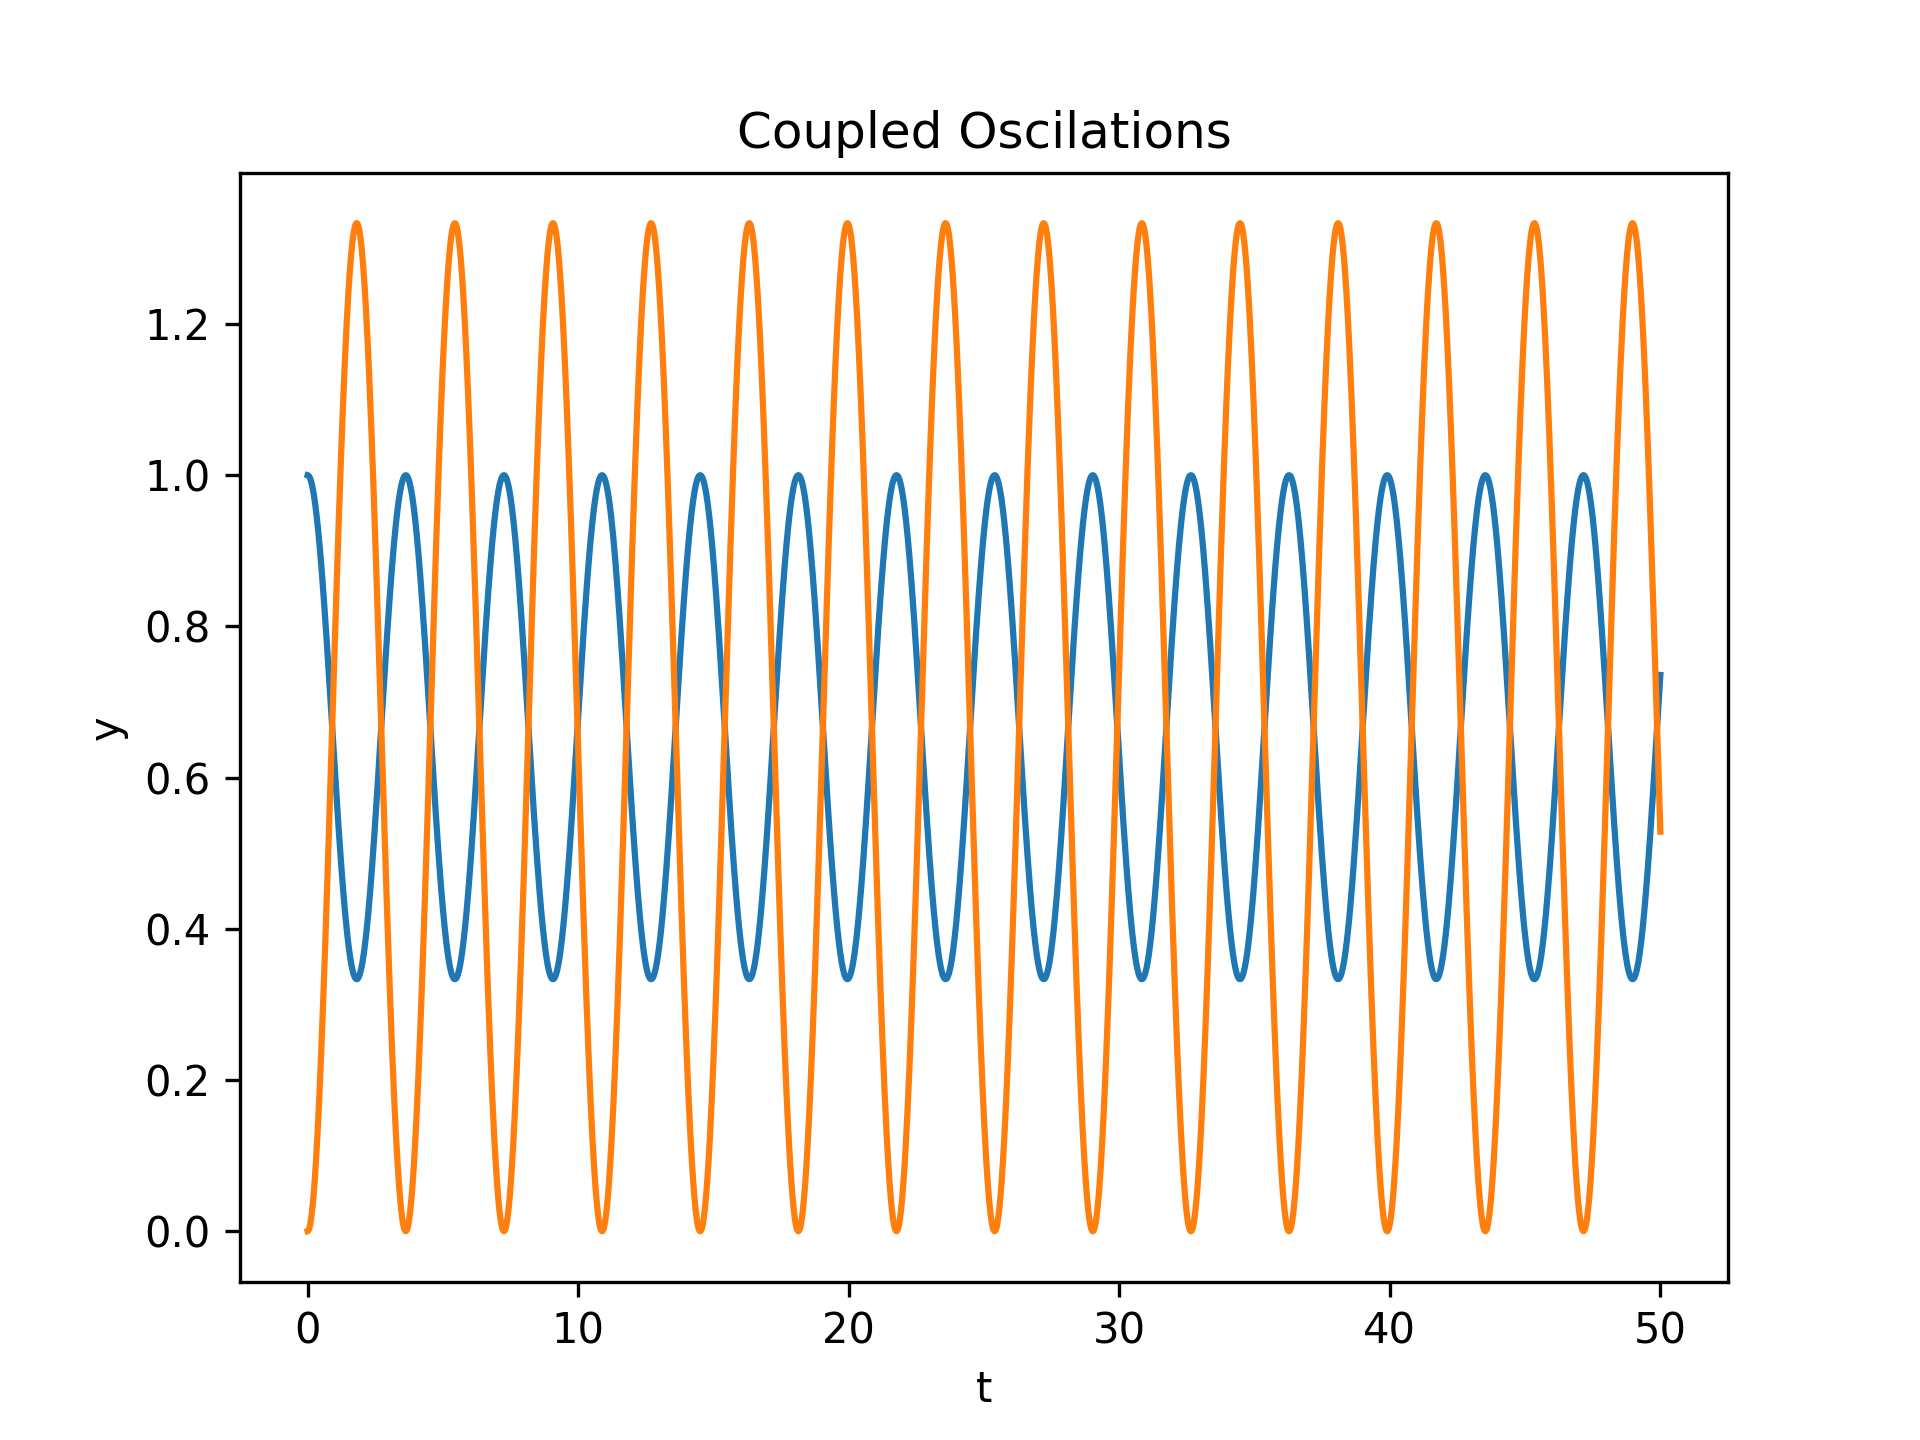
\includegraphics[scale=0.8]{assgn7_plot8.png} 
\caption{Coupled oscillations}
\label{fig8}
\end{figure}

We notice that the outputs of this system are 2 sinusoids which are out of
phase.

\section*{Question 5}
A 2-port RLC filter network is given. We calculate its impulse responses and plot its magnitude and phase responses.

\lstinputlisting[language=Python,firstline=60,lastline=66]{EE19B081_assign7.py}

\begin{figure}[!tbh]
\centering
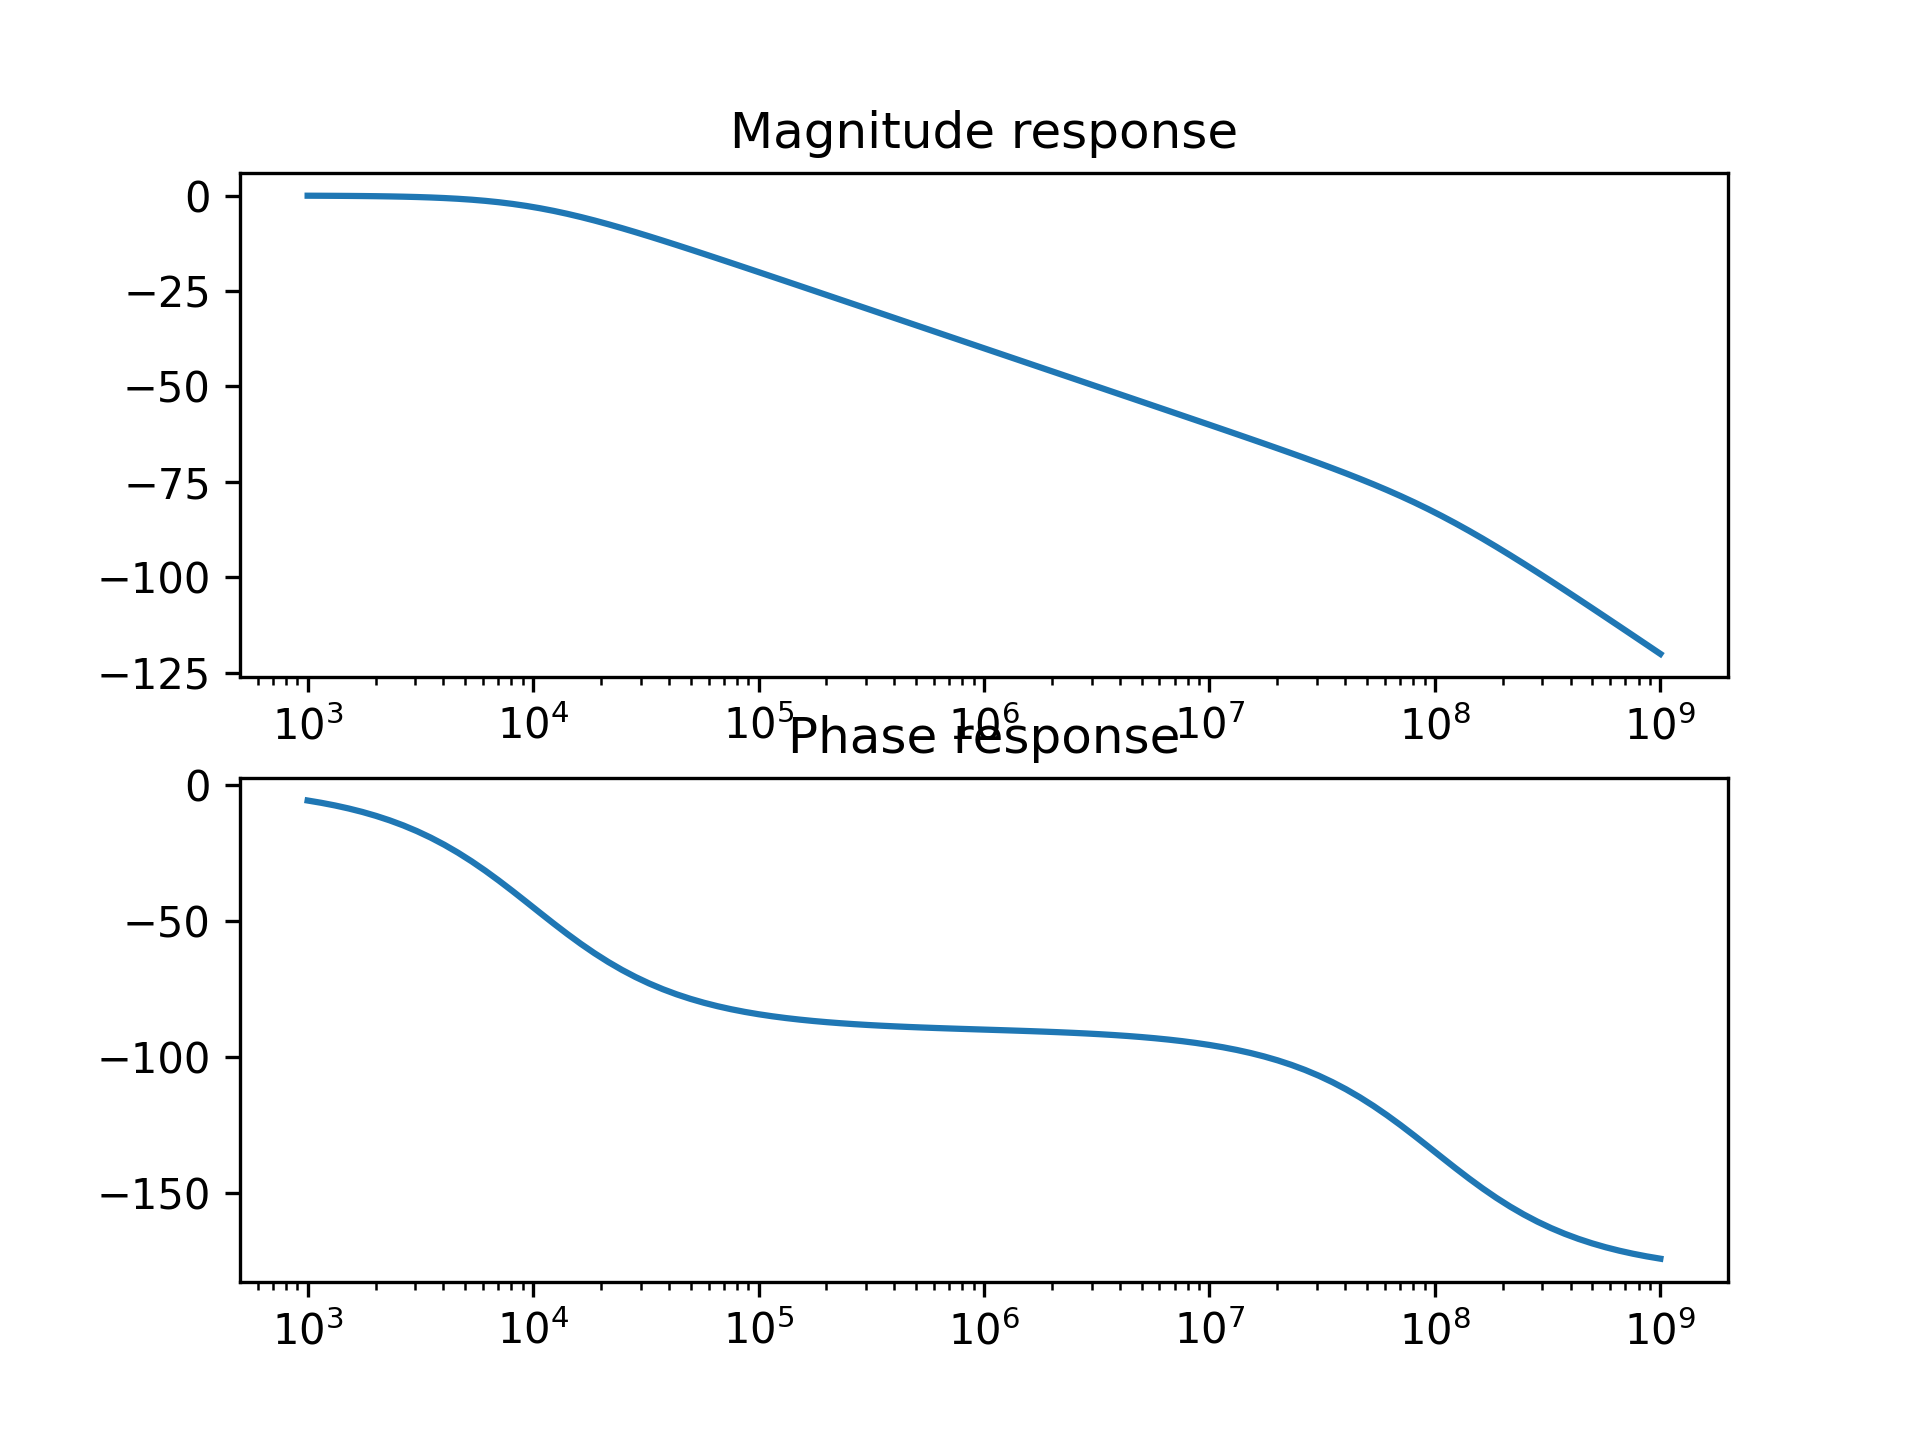
\includegraphics[scale=0.65]{assgn7_plot9.png} 
\caption{Bode plots}
\label{fig9}
\end{figure}

\section*{Question 6}
In the above question , an input signal $V_i$(t) is supplied to the system.
\begin{equation}
	V_i(t) = (cos(10^3t) - cos(10^6t))u(t)
\end{equation}

We obtain the output voltage $V_o$(t) by defining the transfer function as a system and obtaining the output using signal.lsim.

We calculate the output signal for times on different timescales- in microseconds and in milliseconds.

\lstinputlisting[language=Python,firstline=70,lastline=81]{EE19B081_assign7.py}

\begin{figure}[!tbh]
\centering
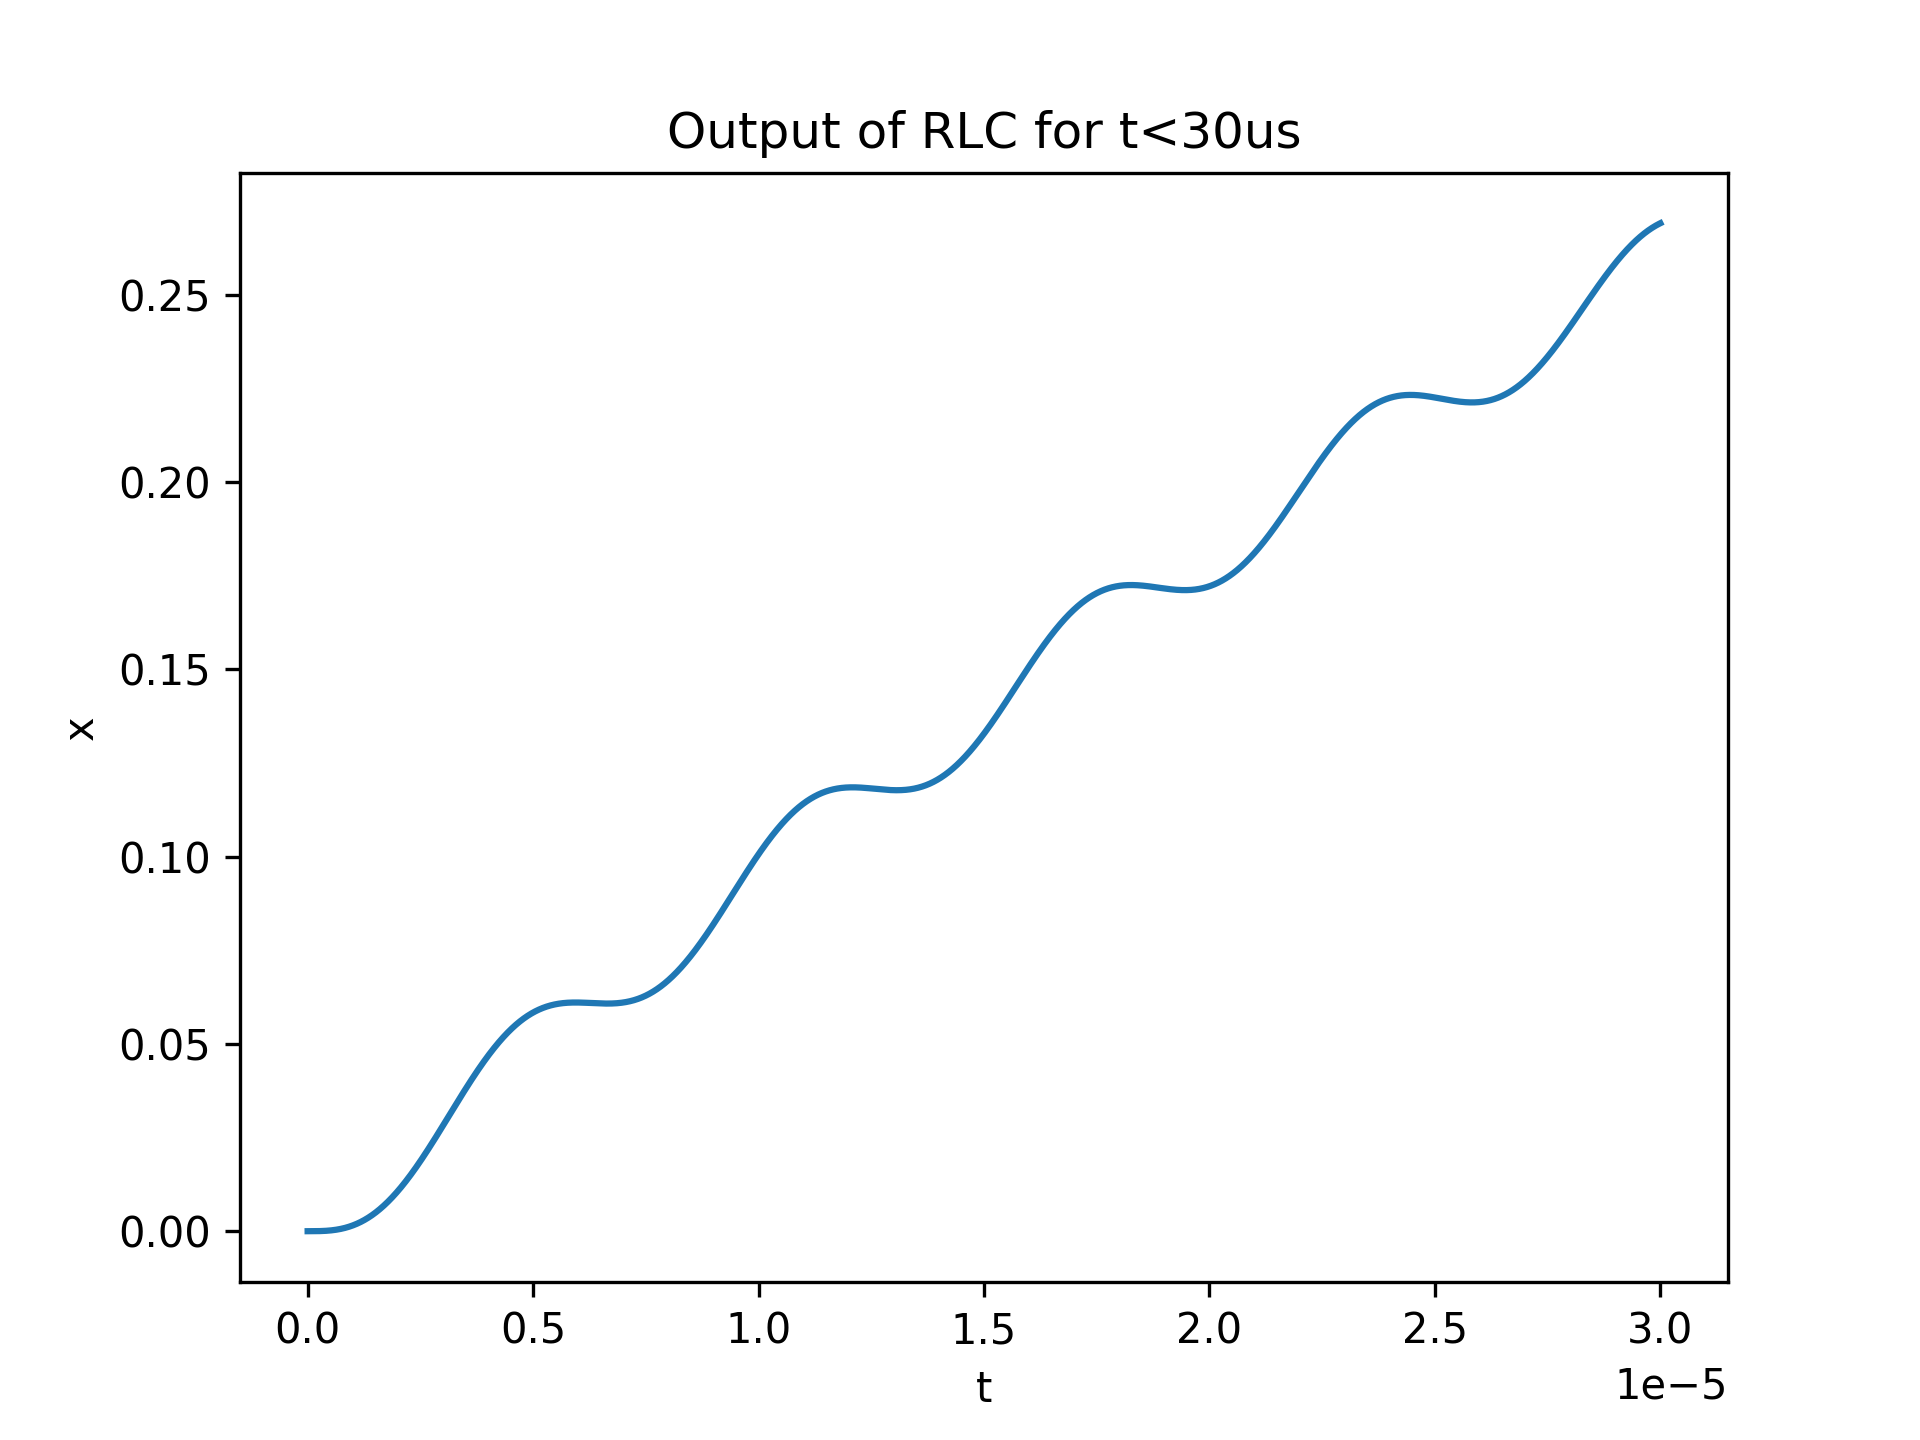
\includegraphics[scale=0.6]{assgn7_plot10.png} 
\caption{Output signal in a timescale of microseconds}
\label{fig10}
\end{figure}

\begin{figure}[!tbh]
\centering
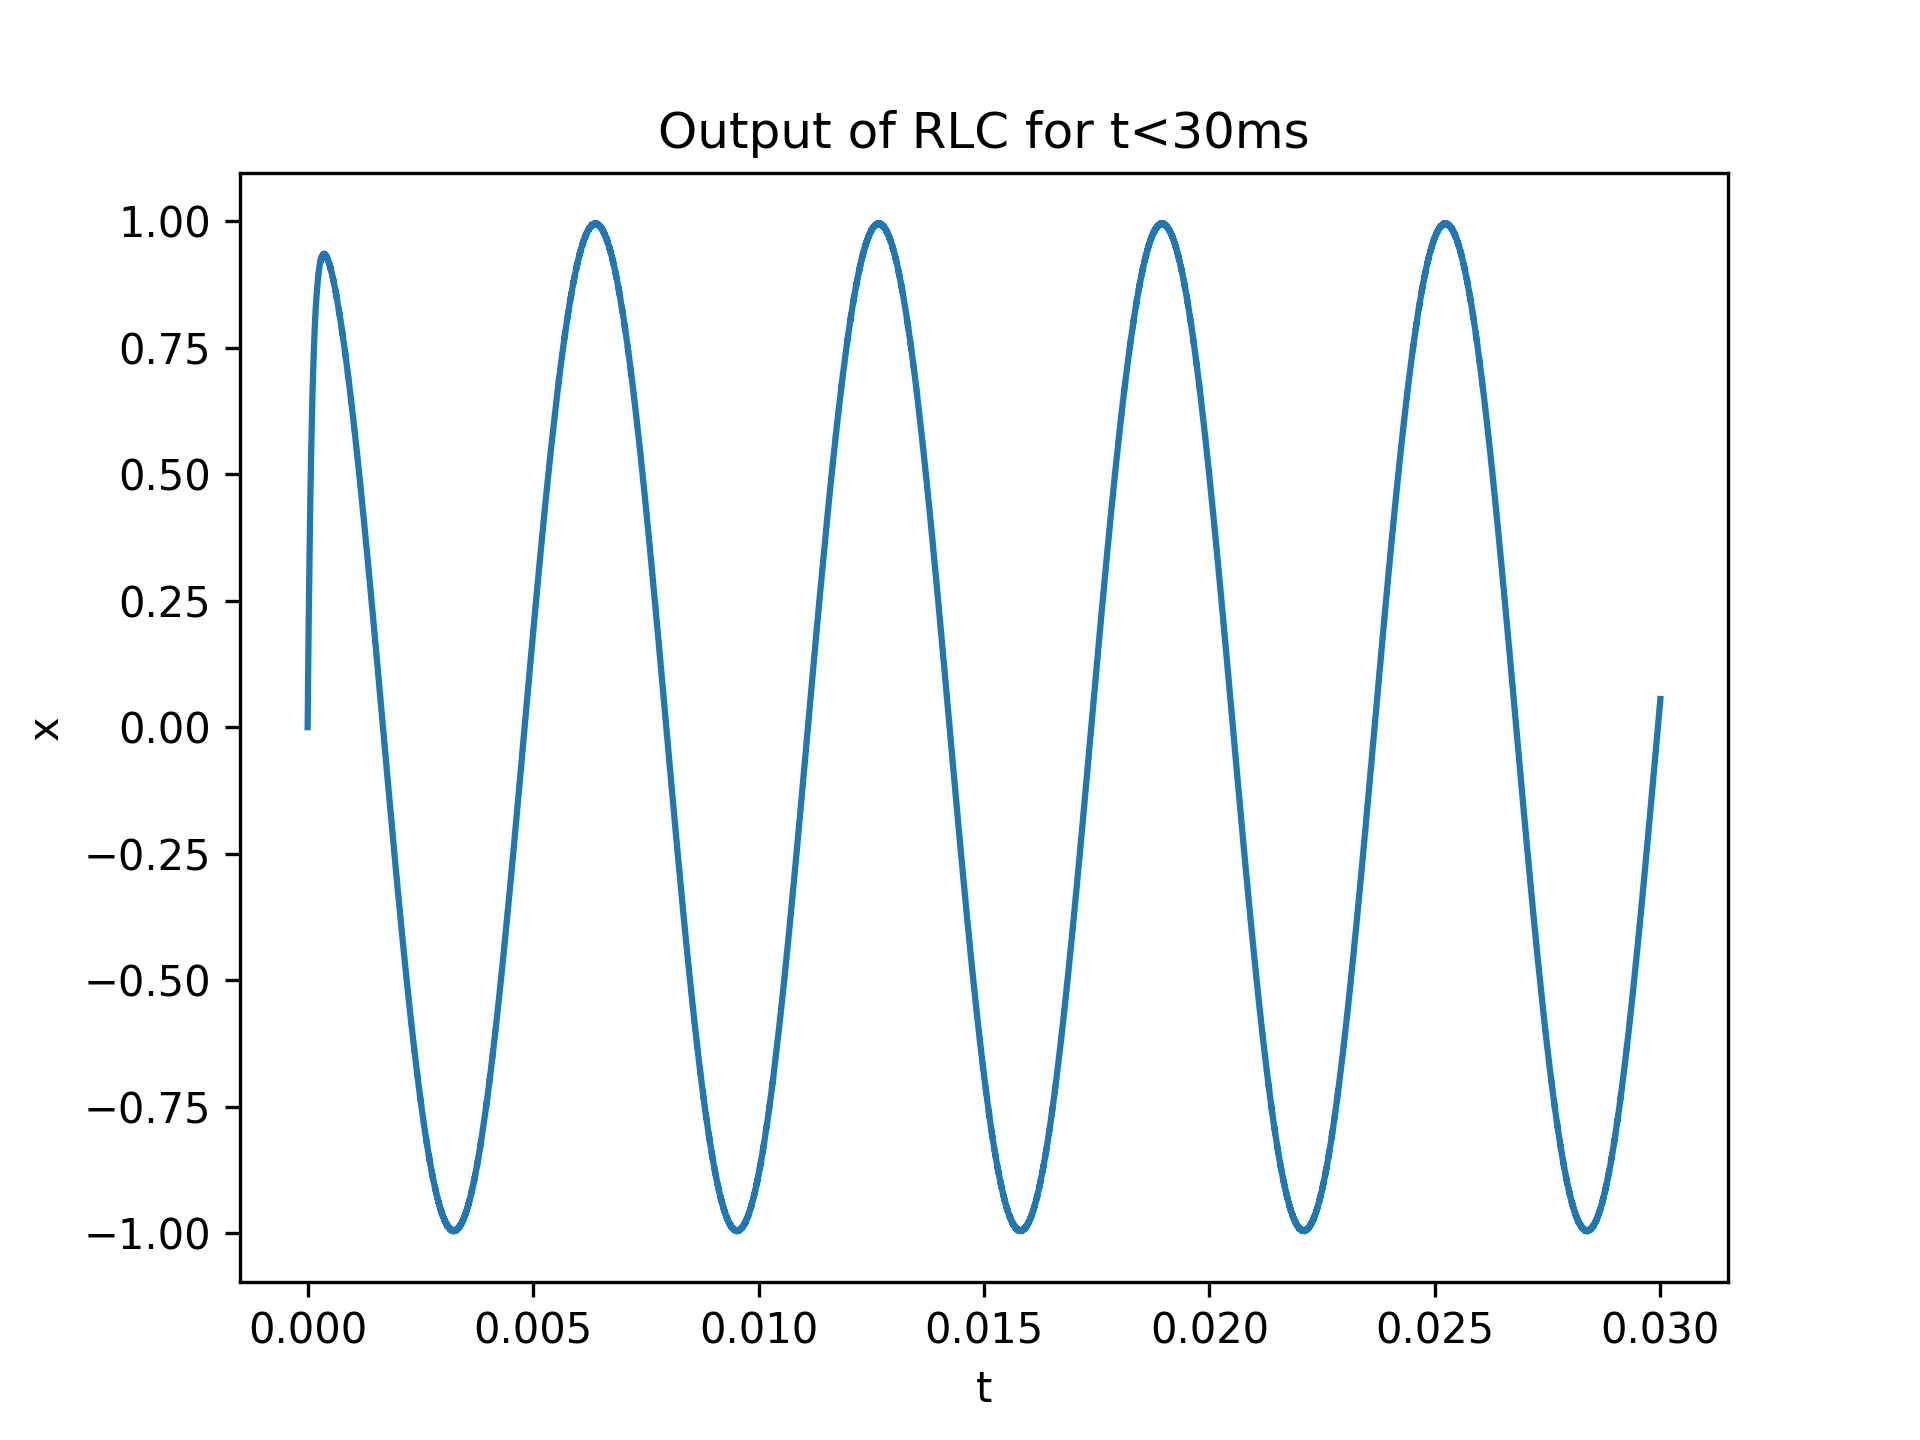
\includegraphics[scale=0.6]{assgn7_plot11.png} 
\caption{Output signal in a timescale of milliseconds}
\label{fig11}
\end{figure}

\section*{Conclusion}
LTI systems are observed in all fields of engineering and are very important.
In this assignment, we have used scipy’s signal processing library to analyze a
wide range of LTI systems.




\end{document}